\subsection{Central Neutron Detector}\label{cnd-section}
The Central Neutron Detector was conceived to extend the CLAS12 acceptance for the recoil neutrons of nDVCS, which are expected to be mostly emitted between $50^{\circ}$ and $70^{\circ}$ \cite{proposal}. The requirements of the detector are:
\begin{itemize}
\item{good capabilities for neutron identification, via the measurement of $\beta$ (with $\beta=\frac{v}{c}$), for the kinematic range of interest ($0.2<p_n<1.2$ GeV/c, $40^o<\theta_n<80^o$)} and
\item{neutron momentum resolution $\sigma_P/P$ within 10\%,}
\end{itemize}
Early simulation studies \cite{proposal} showed that these performances can be achieved by a scintillator-based detector providing a timing resolution of about 150 ps. 

\begin{figure}[ht]
\begin{center}
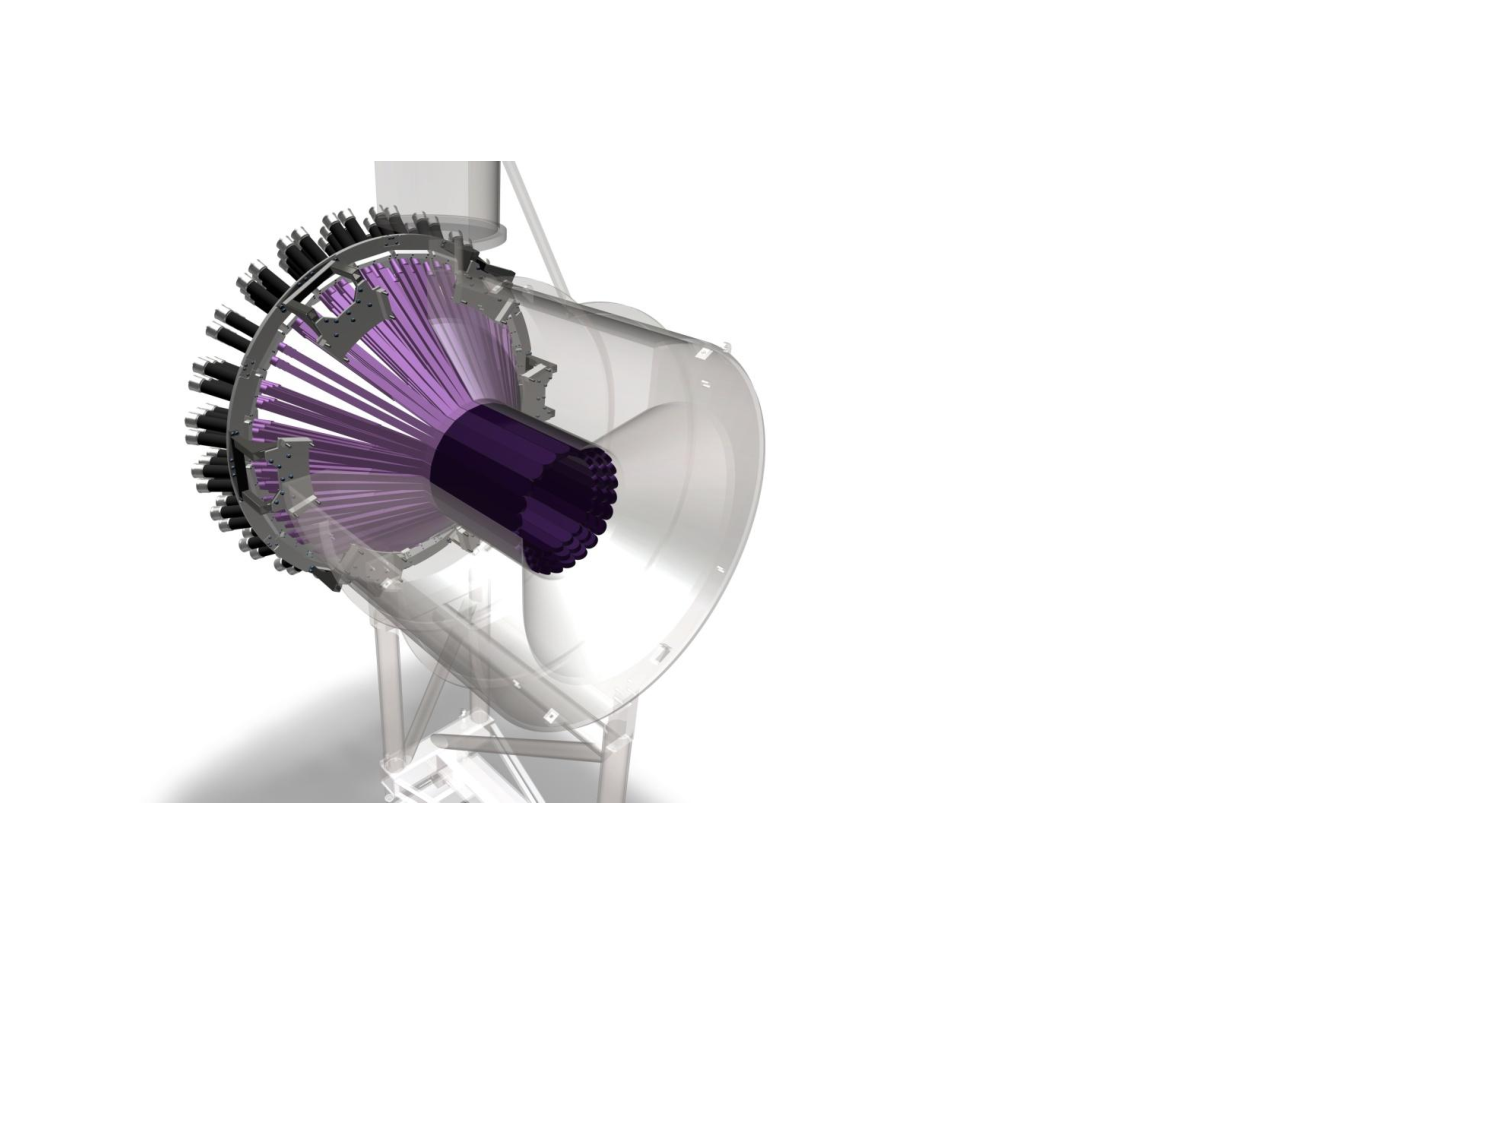
\includegraphics[width=3.5in]{CND_bello.pdf}
\end{center}
\caption [Design of the Central Neutron Detector]
{Design of the Central Neutron Detector, inserted in the CLAS12 solenoid.}
\label{cnd_nice}
\end{figure}

The core of the CND (Fig.~\ref{cnd_nice}), which will be placed in the Central Detector, in the 10 cm of radial space left between the Central Time Of Flight (CTOF) and the solenoid magnet, is a barrel, coaxial with the beam direction, made of three radial layers of trapezoidal plastic-scintillator bars. 
Each radial layer contains 48 bars, connected in pairs by a "u-turn" light guide at the downstream end.
Photomultipliers are coupled to the upstream end of each scintillator via 1.5m-long light guides. For each hit, half of the light emitted in a scintillator paddle is collected by the upstream PMT (the ``direct'' signal), while the other half propagates through the u-turn and the neighboring paddle to the PMT connected at its end (the ``indirect'' signal). 

Three such scintillator pairs (inner, middle, and outer) are grouped together to form a single, radial "block".  The CND comprises 24 of these blocks, covering the entire azimuthal range (Fig.~\ref{CND_Orsay}).

\begin{figure}
\begin{center}
    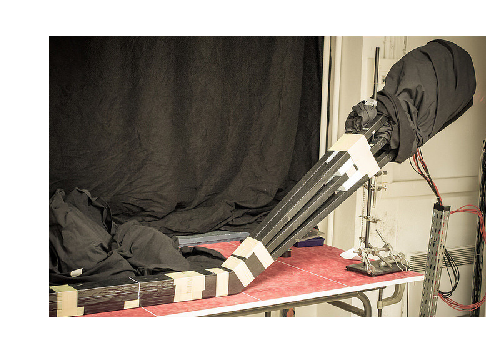
\includegraphics[height=40mm]{block_tested_2.pdf}
    \includegraphics[height=40mm]{cnd_finito.jpg}
  \caption{Construction and testing of the CND at Orsay. Left: one 2x3 block undergoing cosmic ray tests.  Right: all 24 blocks installed into a mock-up of the CLAS12 solenoid.}
  \label{CND_Orsay}
\end{center}
\end{figure}
The assembly of the CND, which was entirely carried out at the IPN Orsay, started in December 2013, and was completed in February 2015. The detector was shipped and stored at JLab in June 2015, awating its installation in CLAS12. Upon assembly, each block of the CND was tested with cosmic rays, triggering on the triple-coincidence of the signal in all three layers. Data were taken for about one week for each block, and the block performances were studied, with special attention to the timing resolution. 
Figure~\ref{tdc_adc_raw} shows the raw distribution of TDCs as a function of ADCs for the six PMTs in one of the 24 blocks. Notice the clear separation between direct (low-TDC/high-ADC) and indirect (high-TDC/low-ADC) signals. 

To define an average time resolution for our setup in the triple-coincidence trigger configuration, we use the method inspired by the work done in \cite{giles} and later adopted for the CLAS TOF system \cite{elton_paper}. 

\begin{figure}
\begin{center}
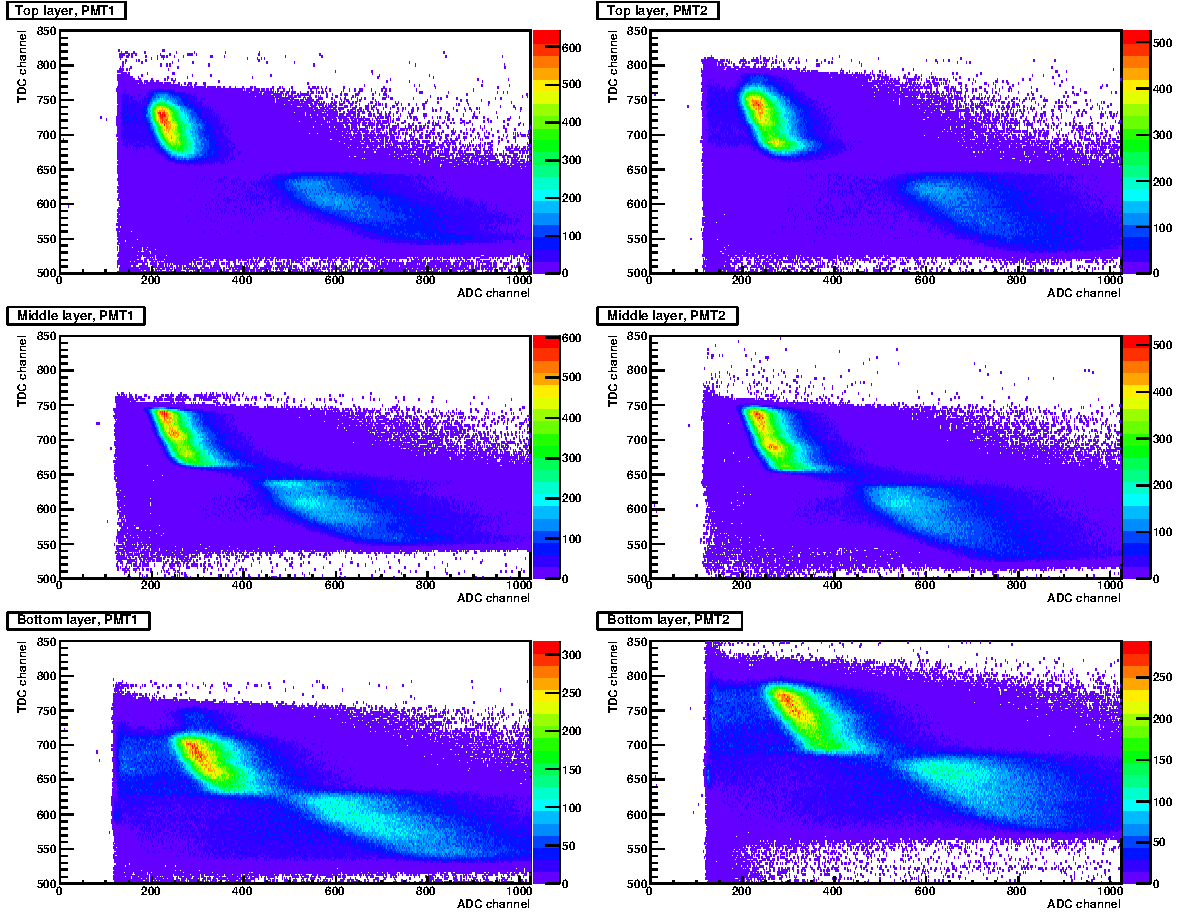
\includegraphics[width=140mm]{tdc_adc_raw.pdf}
\caption[Cosmic ray data for the CND]
{Cosmic rays data. Raw TDC vs ADC for each of the six PMTs of block 2 of the CND. No pedestal subtraction or data-cleaning cuts are applied.}
\label{tdc_adc_raw}
\end{center}
\end{figure}

\begin{figure}
\begin{center}
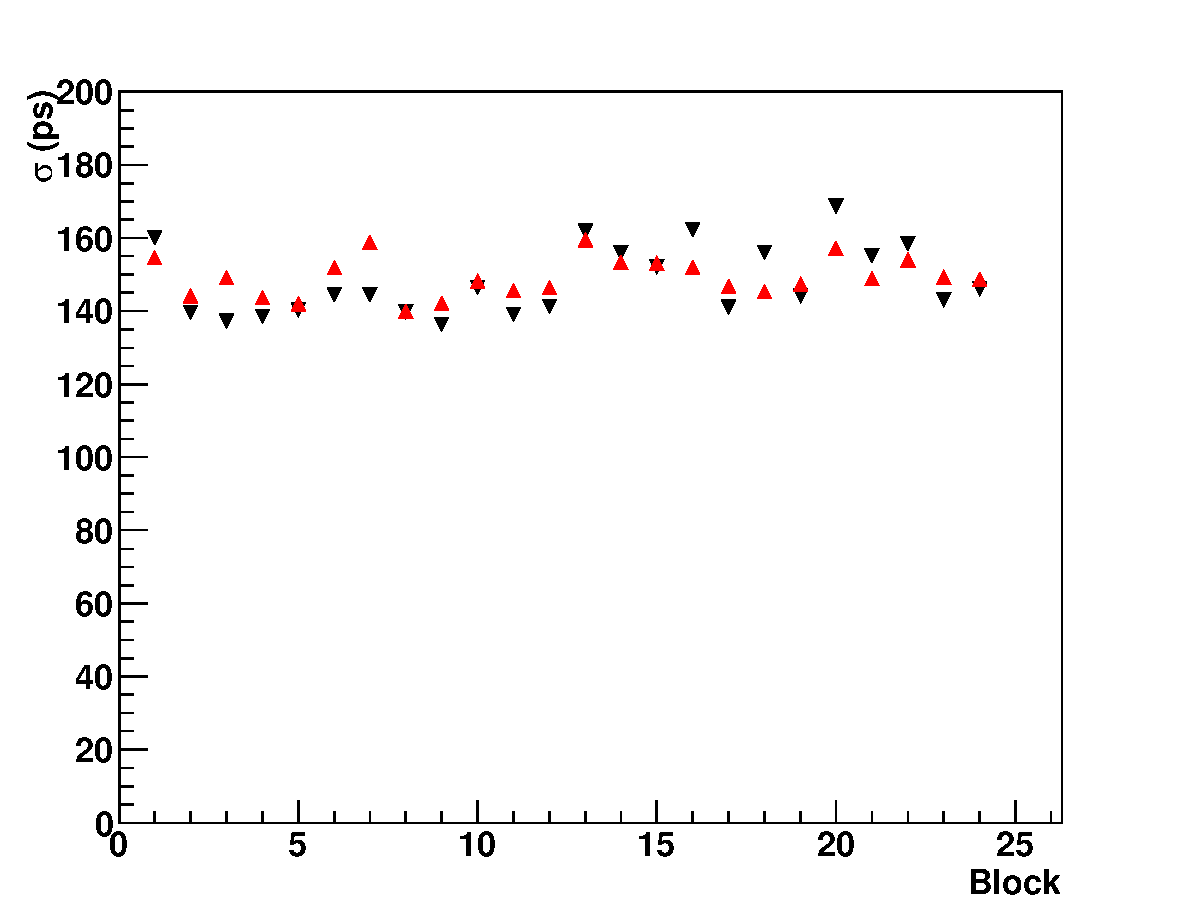
\includegraphics[width=80mm]{res_blocks.pdf}
\caption[Time resolution of the CND]
{Average time resolution for each block of the CND from cosmic rays measurements in triple-coincidence. The black and red triangles are the results obtained with the formulae from, respectively, Refs.~\cite{elton_paper} and \cite{vitali}.}
\label{res_blocks}
\end{center}
\end{figure}

The timing resolutions for all the CND blocks, computed according to the method of \cite{elton_paper}, are represented by the black triangles in Fig.~\ref{res_blocks}. The average is 148.0 ps. As a cross check, the resolution was also computed using the method adopted by V. Baturin for the CLAS12 CTOF \cite{vitali} (red triangles in Fig.~\ref{res_blocks}, with average 149.3 ps). The results of the two methods are consistent. The resolutions of the 24 blocks are very close to the required 150 ps. The systematic uncertainty of our results is estimated to be about $7\%$, determined by repeating the measurements multiple times, and by comparing multiple subsets of each measurement. 

Thus, for resolutions of 150 ps, we have a systematic uncertainty of about 10 ps.

It is also worth mentioning that the TDCs that will be used for the actual experiment will have a better resolution (25ps/channel) than the ones used for these tests (50ps/channel).

\subsection{Simulation and reconstruction}\label{sim_sec}
\begin{figure}[htb]
\begin{center}
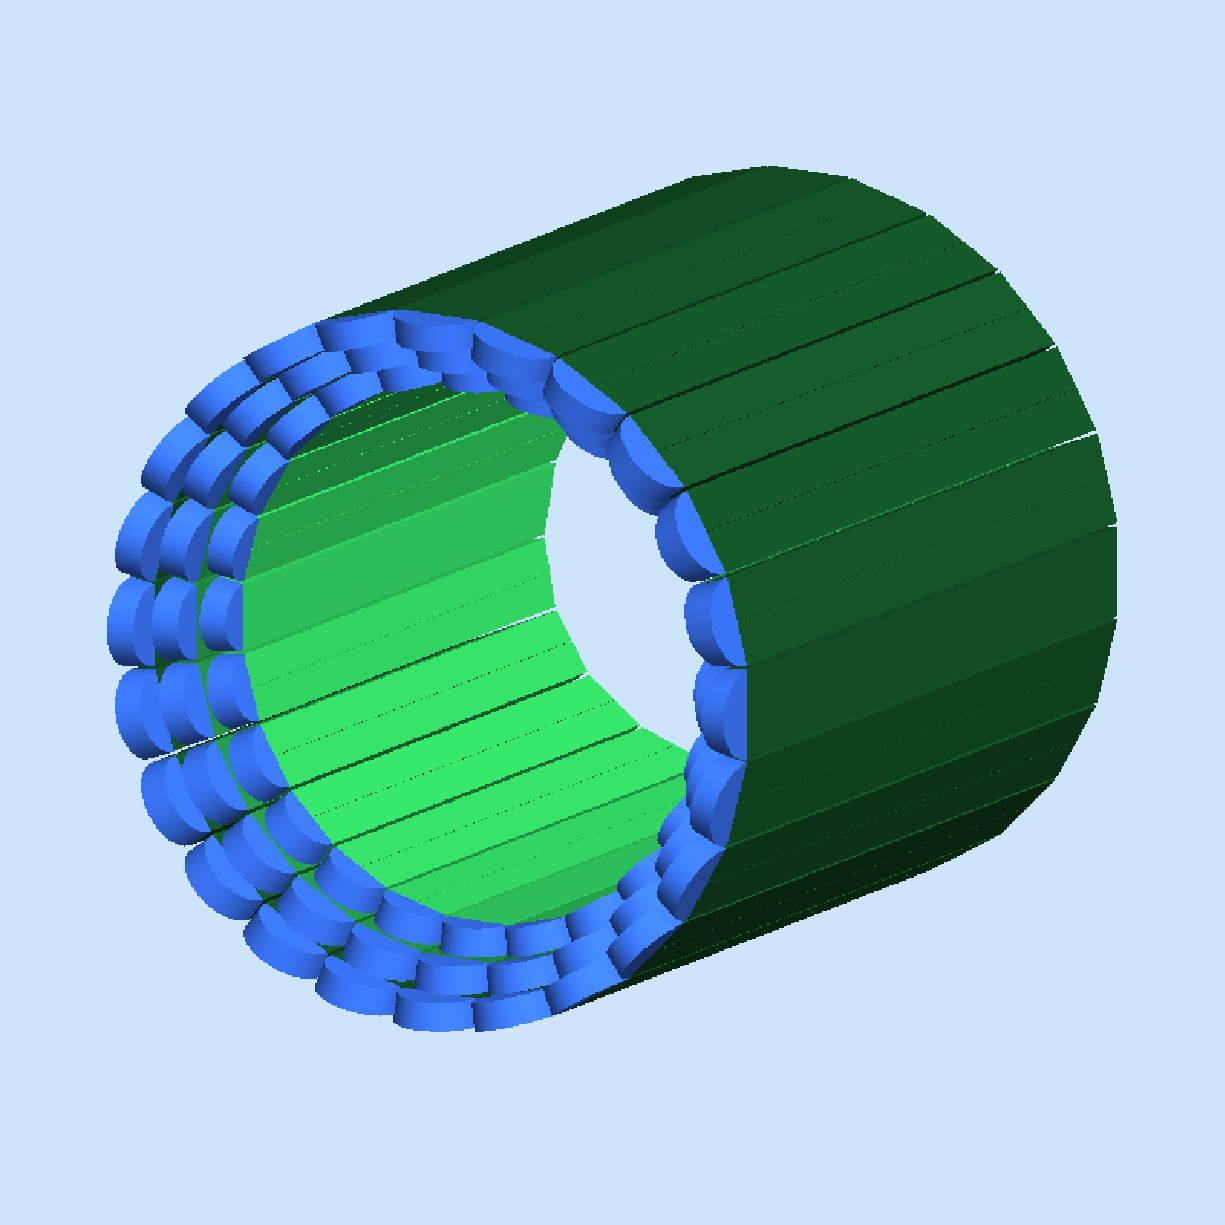
\includegraphics[width=80mm]{CND_4.pdf}
%\vspace{-3.5cm}
\caption {Geometry of the Central Neutron Detector in the GEMC simulation, showing three layers of scintillator paddles (green) coupled in pairs via u-turn light guides (blue) downstream.}
\label{cnd_gemc}
\end{center}
\end{figure}

In order to study the performances of this detector, and thus evaluate the projected results of the nDVCS experiment, its geometry (Fig.~\ref{cnd_gemc}) has been added to the CLAS12 GEANT4-based simulation package, GEMC \cite{mauri}. The energy loss of the particle in the scintillator material is converted to numbers of optical photons in accordance with Birk's formula \cite{birks}, the resulting signal is propagated through the scintillator paddle, light guide and PMT, and the final charge and time are digitized to mimic the output from the ADC/TDC \cite{daria_wiki}.

The timing resolution and the energy loss due to the u-turn geometry have been included in the simulation using the values measured in the cosmic-rays tests described in the previous section. 

Simulations, which included all the other components of the Central Detector, have been run to evaluate the efficiency of the CND for neutrons, its ability to discriminate between neutrons and photons, and its angular and momentum resolutions. Neutrons and photons of momenta varying between 0.1 and 1 GeV/c and having polar angles $\theta$ varying between $50^o$ and $70^o$ have been generated at fixed azimuthal angle ($\phi = 0^o$), pointing to the center of one of the scintillator bars. The results obtained with these simulations are described here below..

\subsubsection{Efficiency}\label{efficiency-section}

 The detection efficiency is defined here as the ratio between the number of events for which a good hit (i.e., a hit having deposited energy above a given threshold) was successfully reconstructed as a neutron in the correct azimuthal bin of the CND and the total number of neutrons generated. 
Several values of energy thresholds, between 1 and 5 MeV, have been tested. 
The efficiency decreases with increasing threshold, and ranges between 12\% at the lowest thresholds and 7\% at the highest ones. 
Figure~\ref{eff_vs_mom} shows the efficiency as a function of the momentum of the neutrons, at a fixed energy threshold of 2 MeV, and for different values of $\theta_n$. 

\begin{figure}[t]  
\begin{center}
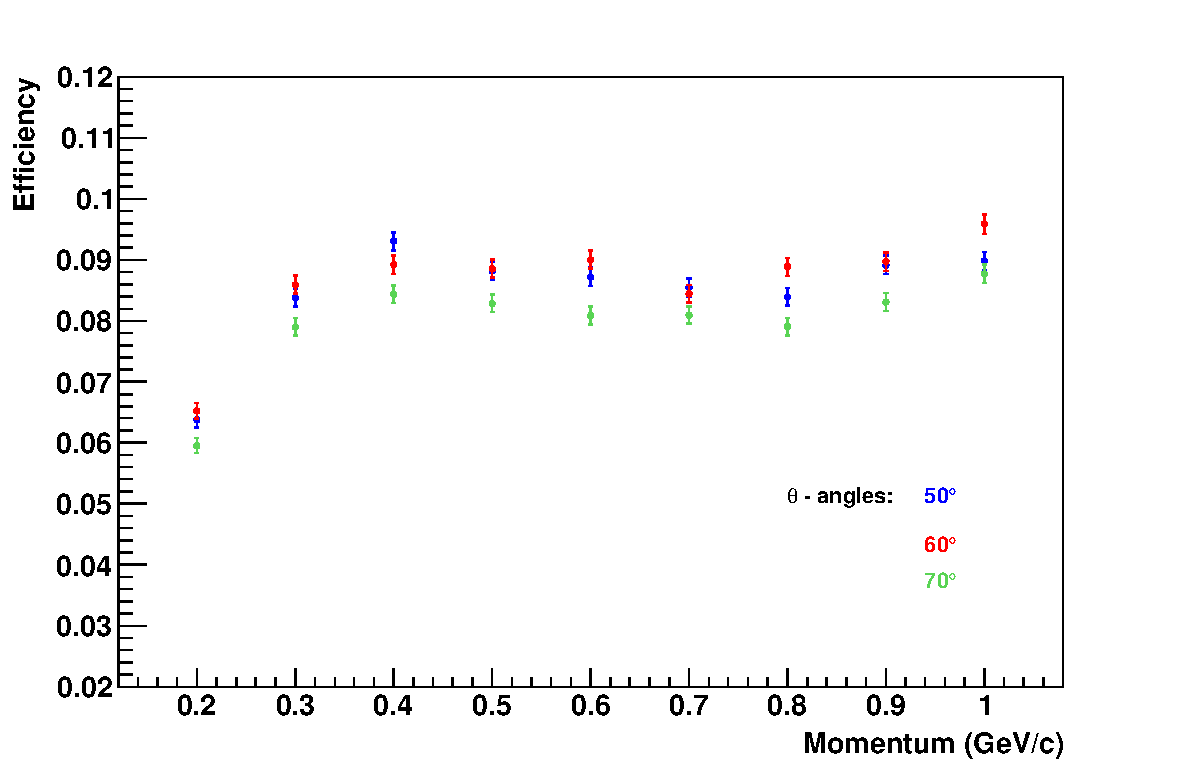
\includegraphics[width=100mm]{eff_vs_mom_diff_theta_II.pdf}
\caption [Neutron detection efficiency as a function of neutron momentum]
{Efficiency for the detection of neutrons, as a function of neutron momentum, for a 2-MeV threshold on the deposited energy. The efficiency is shown for three different values of $\theta_n$, between $50^o$ and $70^o$.
}
\label{eff_vs_mom}
\end{center}
\end{figure}

\subsubsection{Angular and momentum resolutions}\label{resolution-section}

The resolutions on the polar angle $\theta$ of the neutron that can be obtained with the CND are strongly linked to its TOF resolution. The angle $\theta$ is in fact given by
\begin{eqnarray} 
\theta = (180/\pi)\cdot \arccos (\frac{z_{ave}}{l})
\end{eqnarray}
where the reconstructions of the radial distance of the hit from the target, $l$, and of its position along the scintillator bar, $z_{ave}$,  both depend on the time measurement. Using a value deduced from the measurements on the CND prototype to apply a gaussian smearing on the timing \cite{proposal}, 
%\begin{equation}\label{eq_time_smear}
%\sigma_t=\frac{A}{\sqrt{E_{dep}}}, 
%\end{equation}
%(see Appendix~\ref{sec_rec})
the $\theta$ resolution resulting from GEMC was studied as a function of neutron momentum and $\theta$ itself. The results are shown in Fig.~\ref{theta_n_tofcut5}, where the angular resolution $\sigma_\theta$, obtained via gaussian fits of the simulated $\theta$ distributions, is plotted as a function of  $\theta$, for a particular value of neutron momentum (0.4 GeV/c). $\sigma_\theta$ is seen to increase slightly with the angle, from $1.5^{\circ}$ to $3.5^{\circ}$.  It has also been found to be relatively insensitive to the neutron momentum. 

The resolution on the azimuthal angle is directly connected to the total number of scintillator bars along $\phi$. In fact, the bin size $\Delta\phi$ is given by
\begin{eqnarray} 
\Delta\phi = \frac{360^{\circ}}{N}=7.5^{\circ}
\end{eqnarray}
where $N$ is the total number of paddles in $\phi$ (48 for the final design of the CND). $\sigma_\phi$ can be taken as half of $\Delta\phi$, therefore $3.75^o$.
\begin{figure}[hbt]  
\begin{center}
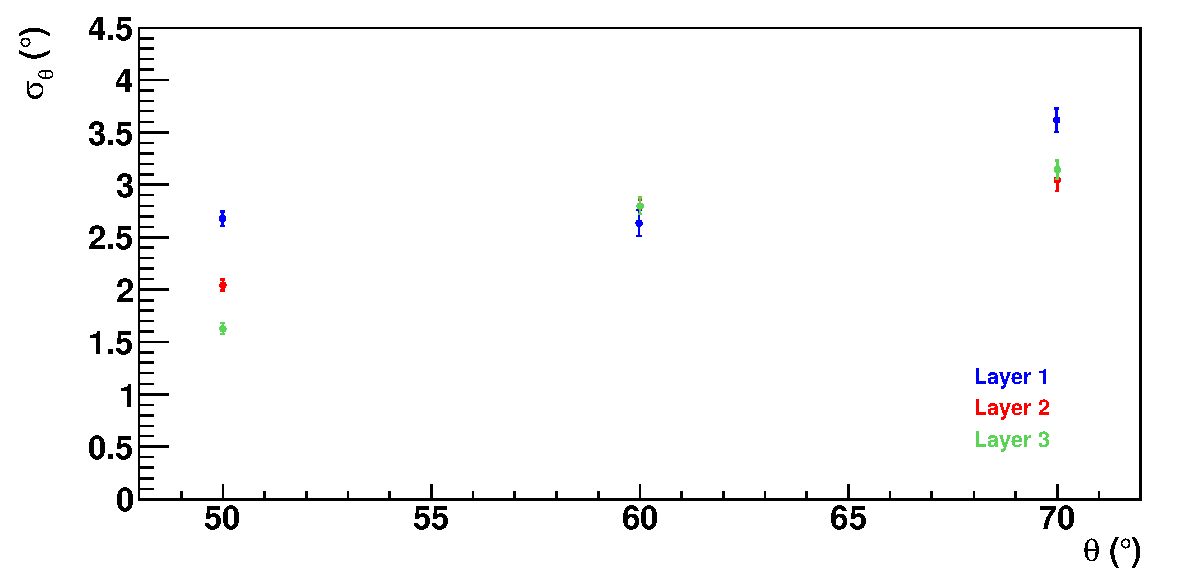
\includegraphics[width=100mm]{sigma_theta_vs_theta_diff_layer.pdf}
\caption [Angular resolution of the CND as a function of $\theta$]
{Angular resolution $\sigma_\theta$ as a function of $\theta$ for neutrons of momentum 0.4 GeV/c, for a 2-MeV threshold on the deposited energy. The three colors of the points correspond to the three radial layers of the CND.}
\label{theta_n_tofcut5}
\end{center}
\end{figure}

\begin{figure}  
\begin{center}
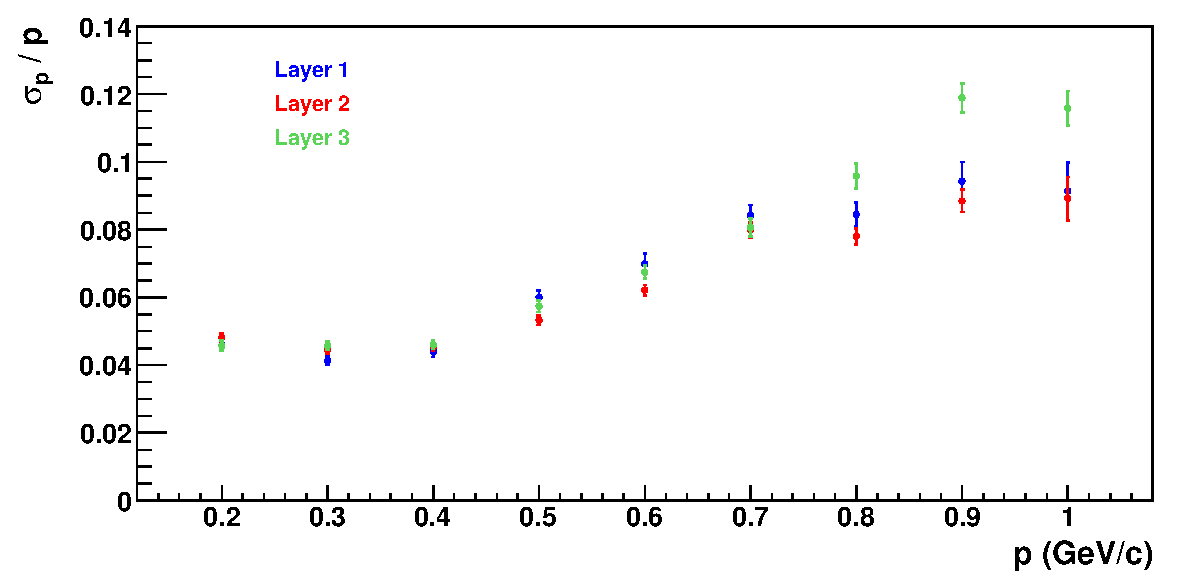
\includegraphics[width=100mm]{mom_res_vs_mom_diff_layers.pdf}
\caption [Momentum resolution as a function of $p$]
{Momentum resolution $\sigma_p/p$ as a function of $p$ for neutrons having $\theta=60^o$, for a 2-MeV threshold on the deposited energy. The three colors of the points correspond to the three radial layers of the CND.}
\label{p_n_tofcut5}
\end{center}
\end{figure}

The resolution on the neutron momentum, calculated after particle identification on the basis of $\beta$, according to the formula
\begin{eqnarray}
p = \frac{\beta\cdot m_n}{\sqrt{1-\beta^2}},
\end{eqnarray}
is also strictly connected to the TOF resolution. Figure \ref{p_n_tofcut5} shows the momentum resolution $\sigma_p/p$ as a function of momentum for neutrons emitted with $\theta=60^o$: it increases with increasing momentum, and ranges between 4\% and 11\%. No appreciable variations of momentum resolution are observed by varying the neutron polar angle.


\subsubsection{Particle Identification}\label{pid-section}

Since the charged particles passing through the CND will be vetoed by the Central Tracker, the only particles that could be mistaken for neutrons in the CND are the photons. 
The efficiency of the CND for detecting photons (Fig.~\ref{eff_photons}) has been estimated in simulations to be similar to that for neutrons, about 10\% for photon energies down to 0.2 GeV.  The efficiency drops to zero for lower energy photons, depending on the threshold cut applied. 

\begin{figure}  
\begin{center}
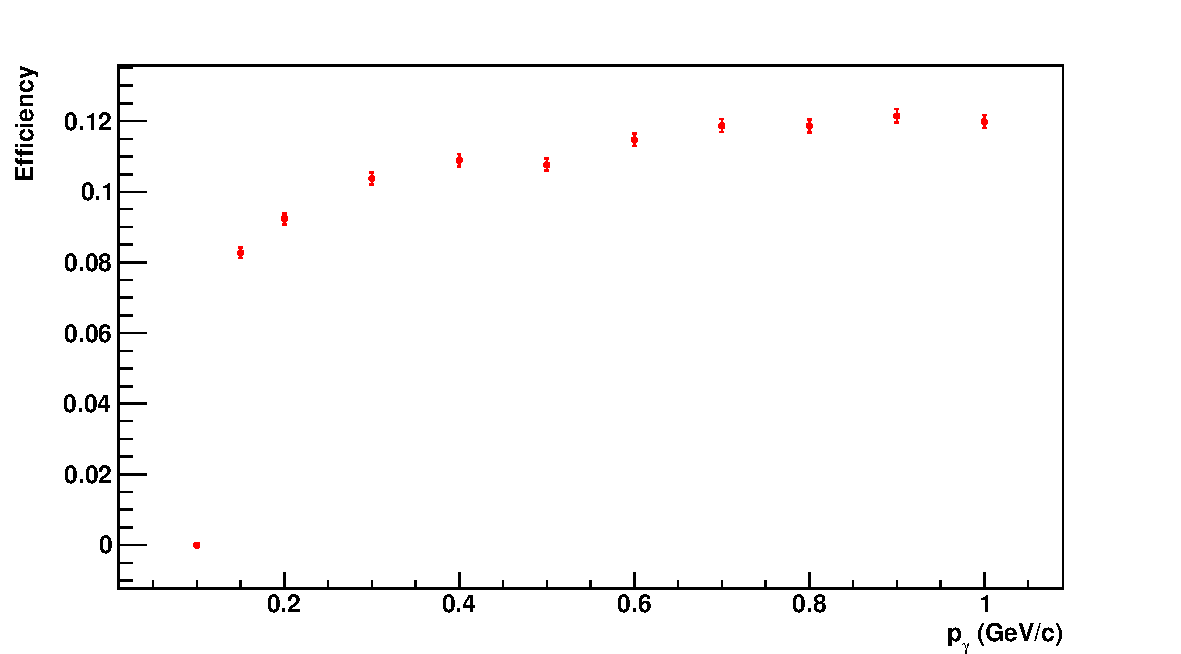
\includegraphics[width=100mm]{efficiency_photons_60deg_new.pdf}
\caption [Photon detection efficiency as a function of photon momentum]
{Efficiency for the detection of photons, as a function of photon momentum, for a 2-MeV threshold on the deposited energy. The efficiency is shown for $\theta_{\gamma}=60^o$. Below $E_\gamma=0.15$ GeV, the photon efficiency drops to zero.}
\label{eff_photons}
\end{center}
\end{figure}

\begin{figure}
\begin{center}
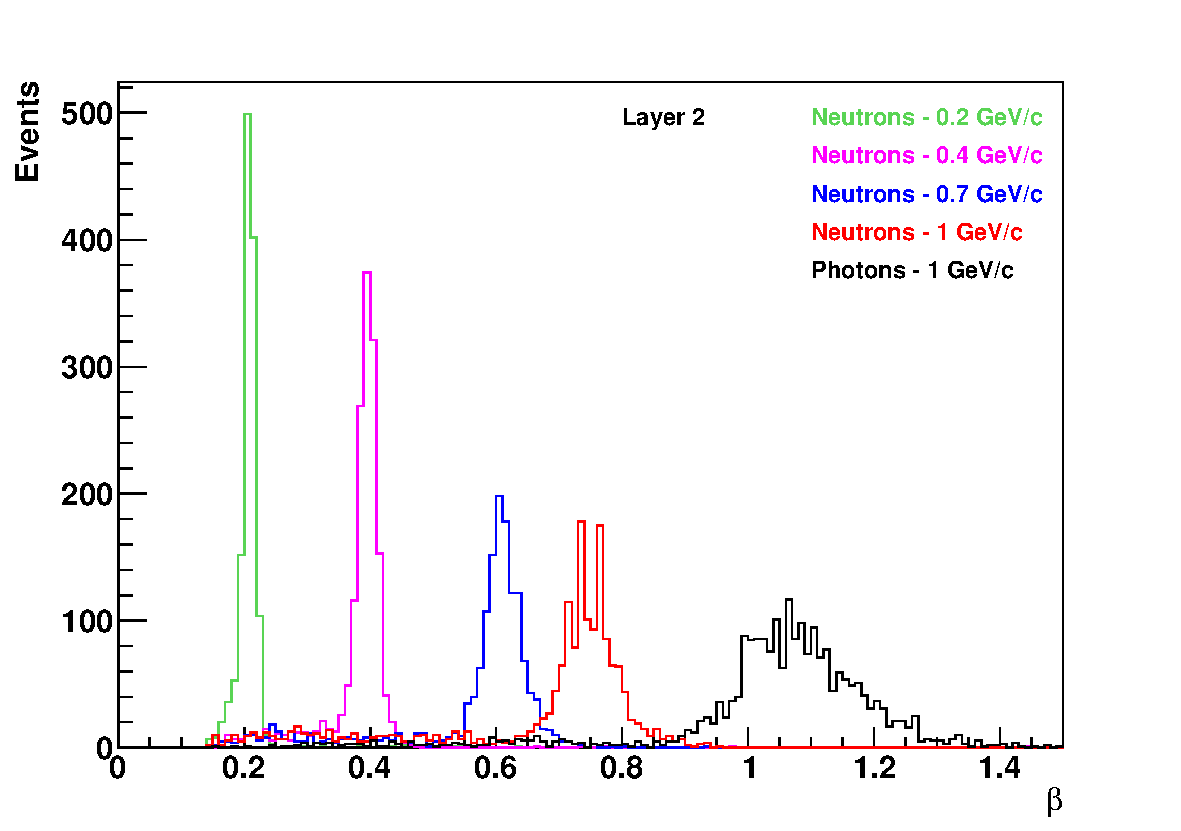
\includegraphics[width=80mm]{beta_comp_layer_2_II.pdf}
\caption [$\beta$ distributions for neutrons and photons in the CND]
{$\beta$ distributions for neutrons with $p_n=0.2$ GeV/c (green), $p_n=0.4$ GeV/c (purple), $p_n=0.7$ GeV/c (blue), $p_n=1$ GeV/c (red), and photons with $E=1$ GeV, for the middle layer of the CND. 
The threshold on the deposited energy is 2 MeV. The plots show all hits, integrated over $\phi$. Equal neutron and photon yields have been assumed here.}
\label{beta_n_g}
\end{center}
\end{figure}

\begin{figure}
\begin{center}
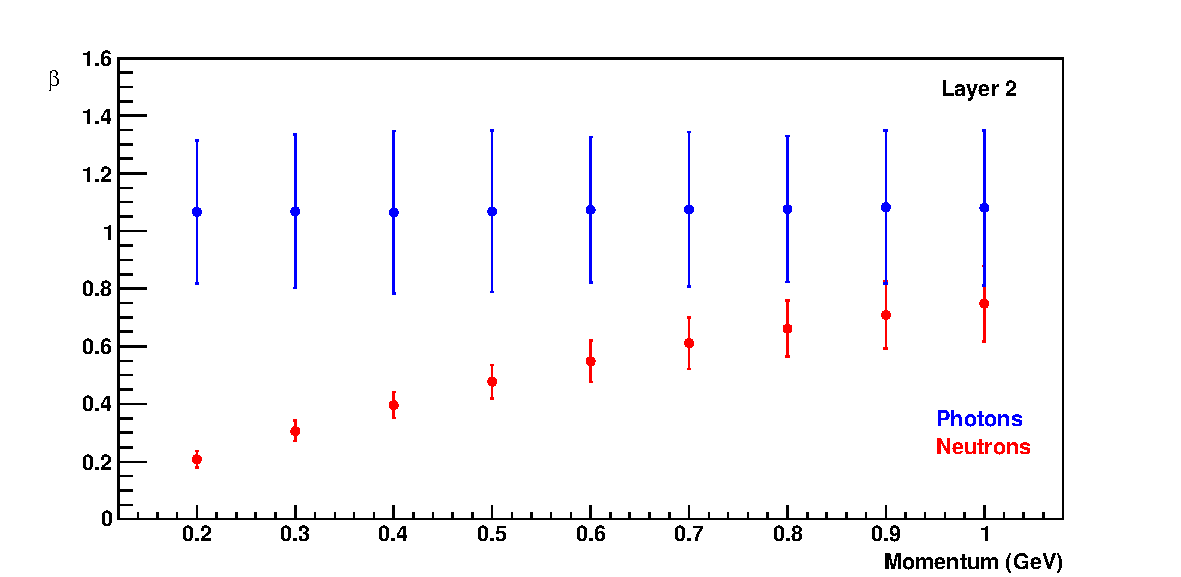
\includegraphics[width=100mm]{beta_res_n_g_comp_L2.pdf}
\caption [$\beta$ versus momentum for neutrons and photons in the CND]
{$\beta$ versus momentum for neutrons (red) and photons (blue) with momenta between 0.2 and 1 GeV, for the middle layer of the CND. The error bars are defined as $3\sigma$, where $\sigma$ is the fitted width of each $\beta$ peak. The threshold on the deposited energy is 2 MeV.}
\label{fig_beta_res}
\end{center}
\end{figure}

Neutrons can be discriminated from photons by means of their $\beta$, and so GEMC simulations have been performed to estimate the $\beta$ distributions that may be obtained from the CND.  Results for one of the three radial layers, integrated over the azimuthal angle, is shown in Figure~\ref{beta_n_g}.  Here $\beta$ distributions for neutrons with momenta between 0.2 and 1 GeV/c are compared with 1 GeV photons.  Very clear separation is evident for neutrons less than about 0.9 GeV/c, which comprise over 90\% of the expected nDVCS events. 

This is evident also from Fig.~\ref{fig_beta_res}, where the error bars correspond to $3 \sigma$, where $\sigma$ is the gaussian width of each $\beta$ distribution. Equal neutrons and photon yields have been assumed for this study. This assumption has been justified with detailed studies on the different types of photonic backgrounds that can affect the CND \cite{proposal}.
